%
% \iffalse
%<*driver>
\ProvidesFile{beamerthemeGotham.dtx}
%</driver>
%<pkg>\ProvidesPackage{beamerthemeGotham}
%<*pkg>
  [2020/09/23 v0.7.0 A beamer theme for the NYU visual identity]
%</pkg>
%<*driver>
\documentclass{ltxdoc}
\EnableCrossrefs
\CodelineIndex
\usepackage{titlesec}
\usepackage{titling}
\usepackage{fontspec}
% Specify different font for section headings
\newfontfamily\headingfont[]{Gotham}
\titleformat*{\section}{\Large\headingfont}
\titleformat*{\subsection}{\large\headingfont}
\titleformat*{\subsubsection}{\headingfont}
\renewcommand{\maketitlehooka}{\headingfont}
\setmainfont{Mercury Text G3 Roman}
\setsansfont{Gotham Book}
\setmonofont{Decima Mono Cyr}
\usepackage{graphicx}
\usepackage{changepage}
\usepackage{hyperref}
\begin{document}
  \DocInput{beamerthemeGotham.dtx}
\end{document}
%</driver>
% \fi
%
% \GetFileInfo{beamerthemeGotham.dtx}
% \title{A Beamer Theme for the NYU Visual Identity}
% \author{Matthew Leingang\thanks{leingang@nyu.edu}}
% \date{\fileversion, Released \filedate}
% \maketitle
%
% \begin{abstract}
% This is the documentation of the \texttt{Gotham} theme for the beamer package.
% \end{abstract}
%
% \changes{v0.2.0}{2019/12/11}{Fixed fonts to the official family}
% \changes{v0.1.0}{2019/12/10}{First working release}
%
% \section{Introduction}
%
% This beamer theme is designed to align with the \href{https://www.nyu.edu/employees/resources-and-services/media-and-communications/styleguide.html}{NYU visual identity}.
% It uses the color palette from the \href{https://www.nyu.edu/employees/resources-and-services/media-and-communications/styleguide/website/graphic-visual-design.html}{NYU website}.
% It uses the Gotham family of fonts.
%
%
% \subsection{Option}
%
% The \textbf{Hoefler} option makes sure that the proprietary fonts are selected, namely
% Gotham.  This can be purchased for \$199 from Hoefler\&Co.
%
% Wihout the option, the \textsf{arev} package is loaded.  It installs Vera Sans as
% the sans serif family, which is a pretty good approximation to Gotham
% (Figure~\ref{fig-arev-v-hoefler})
%
% \begin{figure}
%     \centering
%     \fbox{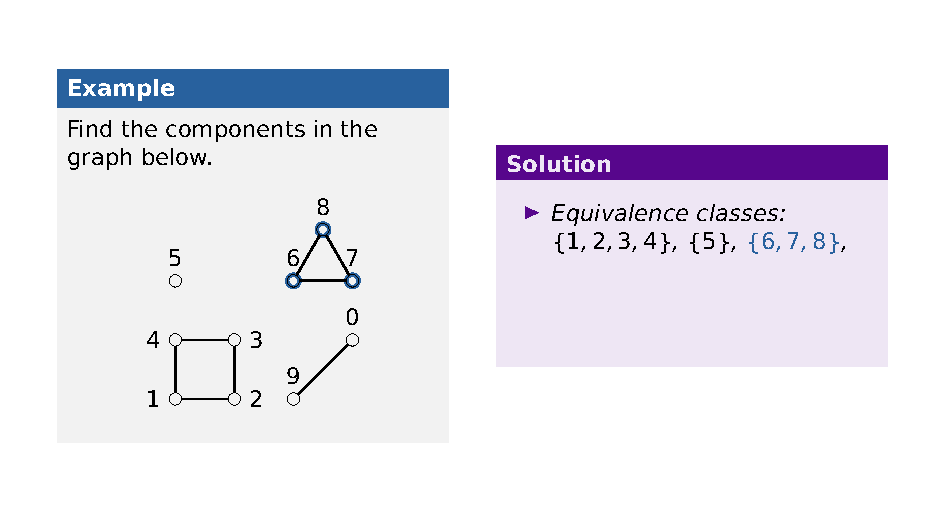
\includegraphics[width=0.9\textwidth]{sample2p45}}\\[2ex]
%     \fbox{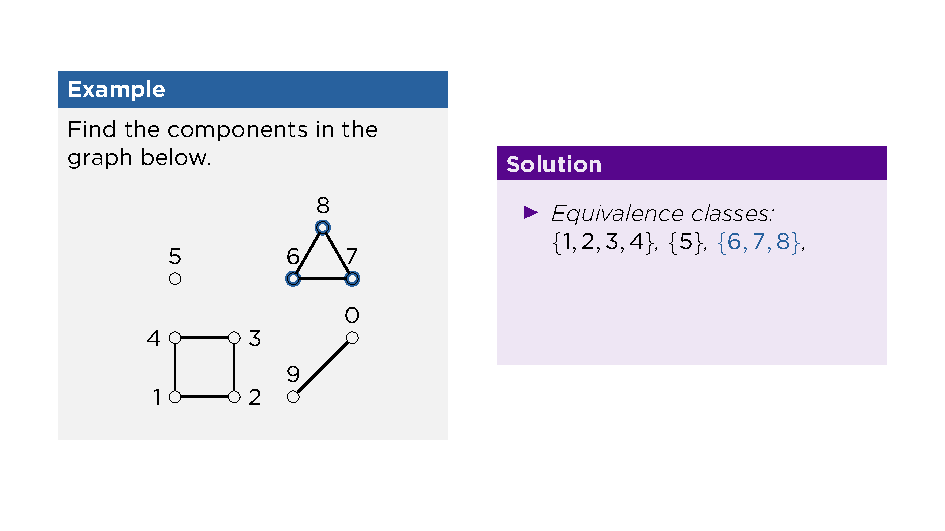
\includegraphics[width=0.9\textwidth]{sample2hp45}}
%   \caption{The same slide in the \texttt{Gotham} theme, with and without the 
%       \textbf{Hoefler} option}
%   \label{fig-arev-v-hoefler}
% \end{figure}
%
% \subsection{Outer theme elements}
% \subsubsection{Logo on title page}
% \changes{unreleased}{2020/09/24}{Added this feature}
% 
% In the “Academic” NYU theme, there is a logo on the title page.  
% The default positioning of the logo is as on the official page,
% but it can also be placed elsewhere.
%
% \begin{itemize}
%     \item \verb|\setbeamertemplate{title page logo}[default]| will 
%           position the logo at the center of the line, below the title,
%           author, and date.  This default template option is selected
%           by default.
%
%     \item \verb|\setbeamertemplate{title page logo}[south west]| will 
%           position the logo at the lower left corner of the title page.
% \end{itemize}
%
% In article mode, \verb|\setbeamertemplate{title page logo}[north west]|
% position the logo at the upper left corner of the first page (or wherever
% \verb|\maketitle| is used).
% 
% Note that because these templates use some TikZ-trickery, your documents
% may need an second run of \LaTeX{} to compile.  But this is almost always
% the case if you've got any labeled and referenced element, or a table 
% of contents, or a bibliography.
%
% Speaking of logos, the bundle including this theme installs many NYU logos
% in \TeX's search tree.  The default is the NYU “short” logo.  You can
% get a Courant one with 
% \verb|\pgfdeclareimage{logo}{courant_short_black}|
%
% \StopEventually{}
%
% \section{Implementation}
%
%    \begin{macrocode}
%<*pkg>
%    \end{macrocode}
%
% \subsection{Option}
%
% \changes{v0.6.0}{2019/12/13}{Added this option}
%
%    \begin{macrocode}
\newif\ifhoefler
\hoeflerfalse
\DeclareOption{Hoefler}{\hoeflertrue}
\ProcessOptions\relax
%    \end{macrocode}
%
% \subsection{Outer theme elements}
%
%    \begin{macrocode}
%\useoutertheme{infolines}
\setbeamertemplate{navigation symbols}{}

\AtBeginPart{\frame{\partpage}}
\AtBeginSection[] % Do nothing for \subsection* 
{ 
  \begin{frame}<beamer|handout> 
  \frametitle{Outline} 
  \tableofcontents[currentsection,currentsubsection] 
  \end{frame} 
}
\AtBeginPart{\frame{\partpage}} 
%    \end{macrocode}
%
% \subsubsection{Logo on title page only}
%
% I'm following NYU's “academic” presentation theme, which has a logo on the
% title page alone.  They put it in the vertical center, below the title and 
% author.  I kind of prefer it in the lower-left corner.
%
% \verb|\setbeamertemplate{title page logo}[south west]| will put the logo
% in the lower-left corner.  
%
%    \begin{macrocode}
\setbeamertemplate{sidebar right}{}
\RequirePackage{tikz}
\tikzset{title page logo/.style={}}
\def\inserttitlepagelogo{\tikz[title page logo]{\node{\pgfuseimage{logo}};}}
\defbeamertemplate<all>{title page logo}{none}{}
\defbeamertemplate<presentation>*{title page logo}{default}{\hfill\inserttitlepagelogo\hfill\null}
\defbeamertemplate<presentation>{title page logo}{south west}{
    \tikzset{title page logo/.append style={remember picture,overlay,
        every node/.append style={
        anchor=south west,
        at={([xshift=1mm,yshift=2pt]current page.south west)}
    }}}
    \inserttitlepagelogo%
}

\defbeamertemplate<article>{title page logo}{north west}{
    \tikzset{title page logo/.append style={remember picture,overlay,
        every node/.append style={
        anchor=north west,
        at={([xshift=0.5in,yshift=-0.5in]current page.north west)}
    }}}
    \inserttitlepagelogo%
}
\addtobeamertemplate{title page}{}{\usebeamertemplate{title page logo}}
\mode<article>{\apptocmd{\maketitle}{\usebeamertemplate{title page logo}}}

\pgfdeclareimage{logo}{nyu_short_black}
\logo{\pgfuseimage{logo}}
%    \end{macrocode}
%
%
%
% \subsection{Color theme elements}
% \changes{v0.6.1}{2020/09/21}{Changed the alert color to orange}
% 
% This package (another module in this bundle) sets some NYU colors
%    \begin{macrocode}
\RequirePackage{xcolor-nyu}
%    \end{macrocode}
%
% Set the palette, structure, example, and alert (warning colors).
% \changes{v0.6.1}{2020/09/22}{Added two more alert colors for success (green) and information (orange).}
%
%     \begin{macrocode}
\mode<presentation>
\setbeamertemplate{headline}[default]

% Palette colors do not have backgrounds
\setbeamercolor{palette primary}{fg=nyupurple1}
\setbeamercolor{palette secondary}{fg=nyupurple2}
\setbeamercolor{palette tertiary}{fg=nyudarkblue}
\setbeamercolor{palette quartenary}{fg=nyulightblue}


\setbeamercolor*{structure}{fg=nyupurple}
\setbeamercolor*{example text}{fg=nyudarkblue}
\setbeamercolor{alert warning}{fg=nyured}
\setbeamercolor{alert information}{fg=nyuorange}
\setbeamercolor{alert success}{fg=nyugreen}
\setbeamercolor*{alerted text}{parent=alert warning}

\setbeamercolor{titlelike}{fg=black}

\setbeamercolor{block title}{fg=nyupurple!10!white,bg=nyupurple}
\setbeamercolor{block title alerted}{use=alerted text,fg=alerted text.fg!10,bg=alerted text.fg}
\setbeamercolor{block title example}{use=example text,fg=white,bg=nyudarkblue}

\setbeamercolor{block body}{parent=normal text,use=block title,bg=block title.fg}
\setbeamercolor{block body alerted}{parent=normal text,use=block title alerted,bg=block title alerted.bg!25!bg}
\setbeamercolor{block body example}{parent=normal text,use=block title example,bg=nyugray4}
\setbeamercolor{block body solution}{parent=normal text,use=block title,bg=block title.fg}

  
% not using a sidebar yet so I don't know what to do with these
\setbeamercolor{sidebar}{bg=nyupurple}
\setbeamercolor{palette sidebar primary}{fg=white,bg=nyupurple}
\setbeamercolor{palette sidebar secondary}{fg=white,bg=nyupurple2}
\setbeamercolor{palette sidebar tertiary}{fg=white,bg=nyudarkblue}
\setbeamercolor{palette sidebar quaternary}{fg=white,bg=nyulightblue}

\setbeamercolor*{separation line}{}
\setbeamercolor*{fine separation line}{}

% Links get colored from the palette too
\AtBeginDocument{
    \hypersetup{colorlinks=true}
    \usebeamercolor{palette primary}
    \hypersetup{linkcolor=fg}
    \usebeamercolor{palette secondary}
    \hypersetup{filecolor=fg,urlcolor=fg}
    \usebeamercolor{palette quaternary}
    \hypersetup{citecolor=fg}
}
%    \end{macrocode}
%
% We set up some new blocks to mimic the alert ``warning'' blocks.
%
%    \begin{macrocode}
\mode
<all>  
%    \end{macrocode}
%
% \begin{environment}{infoblock}
% A block for alert with the ``information'' color.
% \changes{v0.6.1}{2020/09/22}{Added this environment}
%    \begin{macrocode}
\newenvironment<>{infoblock}[1]{%
    \setbeamercolor{alerted text}{parent=alert information}%
    \begin{alertblock}#2{#1}}%
{%
    \end{alertblock}}
%    \end{macrocode}
% \end{environment}
%
% \begin{environment}{successblock}
% A block for alert with the ``success'' color.
% \changes{v0.6.1}{2020/09/22}{Added this environment}
%    \begin{macrocode}
\newenvironment<>{successblock}[1]{%
    \setbeamercolor{alerted text}{parent=alert success}%
    \begin{alertblock}#2{#1}}%
{%
    \end{alertblock}}
%    \end{macrocode}
% \end{environment}
%
%
% \subsection{Fonts}
% 
%    \begin{macrocode}
\ifhoefler
  \RequirePackage[no-math]{fontspec}
% This snippet fixes a "You can't use a prefix with '\begingroup'" error that was coming from
% the fontspec package.  
% Thanks to Philippe Goutet.  See \url{http://tex.stackexchange.com/q/5996/1402}.
  \def\alloc@#1#2#3#4#5%
  {\ifnum\count1#1<#4% make sure there's still room
      \allocationnumber\count1#1
      \global\advance\count1#1\@ne
      \global#3#5\allocationnumber
      \wlog{\string#5=\string#2\the\allocationnumber}%
    \else\ifnum#1<6
      \def\etex@dummy@definition{}% <-- code added
      \begingroup \escapechar\m@ne
      \expandafter\alloc@@\expandafter{\string#2}#5%
    \else\errmessage{No room for a new #2}\fi\fi
  }

  \RequirePackage{xltxtra}
  \defaultfontfeatures{Mapping=tex-text}
  \setmainfont[BoldFont=Gotham Bold]{Gotham Book}
  \setmathrm{Cambria Math}
  \setsansfont[BoldFont=Gotham Bold]{Gotham Book}
\else
    \let\emptyset\relax
    \RequirePackage{arev}
    \let\titlefont\sffamily
\fi
%    \end{macrocode}
%
% Neither Gotham nor Arev come with small caps.  So we “fake” it.
% See \url{https://tex.stackexchange.com/a/55733/1402}
%    \begin{macrocode}
\def\fakesc#1{%
  \begingroup%
  \xdef\fake@name{\csname\curr@fontshape/\f@size\endcsname}%
  \fontsize{\fontdimen8\fake@name}{\baselineskip}\selectfont%
  \MakeUppercase{#1}%
  \endgroup%
}
\let\textsc\fakesc
%    \end{macrocode}

%
%    \begin{macrocode}
\usefonttheme[onlylarge]{structurebold}
\setbeamerfont{frametitle}{size=\Huge}
\setbeamerfont{framesubtitle}{size=\Large}
\setbeamerfont{title}{size=\Huge}
\setbeamerfont{block title}{series=\bfseries}
%    \end{macrocode}
%
%    \begin{macrocode}
%</pkg>
%    \end{macrocode}
%
% \Finale
%
